
\FloatBarrier
\section{Система Ресслера} % {{{1 _ROSS_
\label{atu:sect:ross}

\LinkRef{
  ross: ASAU-14. ISDMCI-2011, ISDMCI-2012
  % ~/doc/tex/asau/asau14/atu/atu.tex
}

\subsection{Визначення системи та аналіз її динаміки} % {{{2 _ross_task

Динамічна система Ресслера~(\ref{atu:eq:rossler}) є в певній мірі
абстрактною моделлю, яка описує кінетику коливальних і
хаотичних хімічних процесів~\cite{ROSSLER1976397, neimark_stoch_chaos_vibro,koltsova_nl_dyn_chem,berje_order_in_chaos,chulichkcov_mm_ml_dyn, puhov_ur_reaction_diffusion},
таких як реакція Білоусова-Жаботінського, кристалізація фосфіту свинцю
та інших реакцій.

\begin{equation}
\begin{cases}
  \dot{x}  = -y - z  ,  \\
  \dot{y}  = x + a y ,\\
  \dot{z}  = b + z \cdot ( x-c ) .
\end{cases}
\label{atu:eq:rossler}
\end{equation}

Тут \(x\), \(y\), \(z\) --- змінні стану системи, які відповідають
концентраціям основних реагентів в хімічної
системі, що моделюється.
Відповідно \(a\), \(b\), \(c\) --- параметри, що визначають
динаміку системи, які в хімічної системі визначаються
константами хімічної рівноваги і концентраціями допоміжних реагентів.

При моделюванні даної системи покладемо \(a = 0.25 \), \(b = 1 \). У цьому
випадку параметр \(c \) визначає тип динаміки системи. Визначення
значення даного параметра і буде метою задачі ідентифікації.

У даній системі немає зовнішнього вхідного сигналу \(u (t) \). Це
пояснюється тим, що за рахунок підтримки постійних концентрацій
допоміжних компонент, постійного поповнення початкових речовин і
видалення продуктів реакції система володіє власним джерелом
енергії, який забезпечує динаміку системи і при відсутності
зовнішнього впливу.

Як і інші системи хаотичної динаміки, система Ресслера не
дозволяє побудувати систему ідентифікації, засновану на
формуванні критерію якості ідентифікації як міри близькості
безпосередніх значень вихідних сигналів об'єкта \(x_o (t) \) і моделі
\(x_m (t) \). Більш того, сам вид поведінки даної системи може значно
змінюватися при малих змінах параметрів, здійснюючи перехід
від хаотичного до складно-періодичного і назад.

При малих значеннях параметра (\(c \approx 3 \)) система проявляє
регулярну динаміку, здійснюючи коливальний рух навколо точки
нестійкої рівноваги~(рис.~\ref{atu:f:ross_attractor_0300}).

\begin{figure}[htb!]
  \PicDouble{p/cha/ross/ross0-p_xyz_c=03x50.png}{p/cha/ross/ross_f-p_f_c=03x50.png}
  \caption{Аттрактор~(a) і спектр~(b) системи Ресслера (\ref{atu:eq:rossler}) в режимі регулярних коливань ($c = 3.5$)}
\label{atu:f:ross_attractor_0300}
\end{figure}

При збільшенні значення параметра \(c\) відбувається подвоєння
періоду, поведінка системи стає все більш складною, і в певному
діапазоні значень параметра система демонструє хаотичну
динаміку~\cite{atu_st67} (рис.~\ref{atu:f:ross_attractor_0588}).

\begin{figure}[htb!]
  \PicDouble{p/cha/ross/ross0-p_xyz_c=05x88.png}{p/cha/ross/ross_f-p_f_c=05x88.png}
  \caption{Аттрактор~(a) і спектр~(b) системи Ресслера (\ref{atu:eq:rossler}) в режимі хаотичних коливань ($ c = 5.88 $)}
\label{atu:f:ross_attractor_0588}
\end{figure}


Простежується відміна спектра системи Ресслера в хаотичному
режимі від спектру за аналогічних умов для систем Лоренца. Відмінність
полягає в тому, що існує яскраво виражений пік, відповідний
базовій частоті, а області суцільного спектра характеризуються
невеликою амплітудою. При деяких великих значеннях параметра
$c$ діапазон суцільного спектра стає більш помітним, проте
загальна структура спектра залишається такою~ж.

При подальшому збільшенні значення параметра
\(c\) спостерігаються переходи від хаотичного до
складно-періодичному (рис.~\ref{atu:f:ross_attractor_2500}) і назад.

\begin{figure}[htb!]
  \PicDouble{p/cha/ross/ross0-p_xyz_c=25x00.png}{p/cha/ross/ross_f-p_f_c=25x00.png}
  \caption{Аттрактор~(a) і спектр~(b) системи Ресслера (\ref{atu:eq:rossler}) в режимі складно-періодичних коливань ($ c = 25.0 $)}
\label{atu:f:ross_attractor_2500}
\end{figure}

При цьому спостерігається лінійчатий спектр. Також, при таких
значеннях параметра може стрибкоподібно зміняться розмір області, в яку
вписаний аттрактор. У цьому сенсі система Ресслера потенційно є
більш складною для ідентифікації, ніж системи Лоренца і ``Sprott~A''.

Ділянки хаотичної динаміки перемежовуються з ділянками
складно-періодичних коливань. При цьому відбувається зміна
структури атрактору~\cite{buscarino_sync_rossler, rosalie_rossler_template}. Більш того,
при одному і тому ж типі динаміки може змінюватися як структура
аттрактора, так і розмір області, в яку він може бути вписаний.

% }}}2

\subsection{Аналіз і вибір критеріїв} % {{{2

Система Ресслера відрізняється від уже розглянутих систем
тим, що відповідна фізична (або хімічна) система знаходиться в
умовах, в яких немає сенсу використовувати закон збереження
енергії. Концентрації реагентів, які витрачаються в реакції,
підтримуються на постійному рівні за рахунок зовнішніх
впливів. Також вважається,  що продукти
реакцій, які не використовуються, видаляються.
Такі властивості дають підстави
припускати, що стандартний набір критеріїв, який був
застосований для систем Лоренца і системи ``Sprott~A'', не буде
містити відповідного критерію. Виходячи з форми аттрактора,
що містить близькі до кругових траєкторії поблизу площини
$XY$, додамо критерій
$q_{x^2 + y^2} $ до списку розглянутих. Спостереження за зміною
форми аттрактора при збільшенні параметра
$c$ дозволяють помітити, що, в цілому, максимальна апліката
також зростає. Це спостереження дозволяє додати критерій
$ q_{z \max{}} $ в число розглянутих~\cite{atu_ISDMCI2012, atu_asau14}. Залежності
розглянутих критеріїв від параметра
$ c $ наведені на рис.~\ref{atu:f:ross_q}.


\begin{figure}[htb!]
\begin{center}
  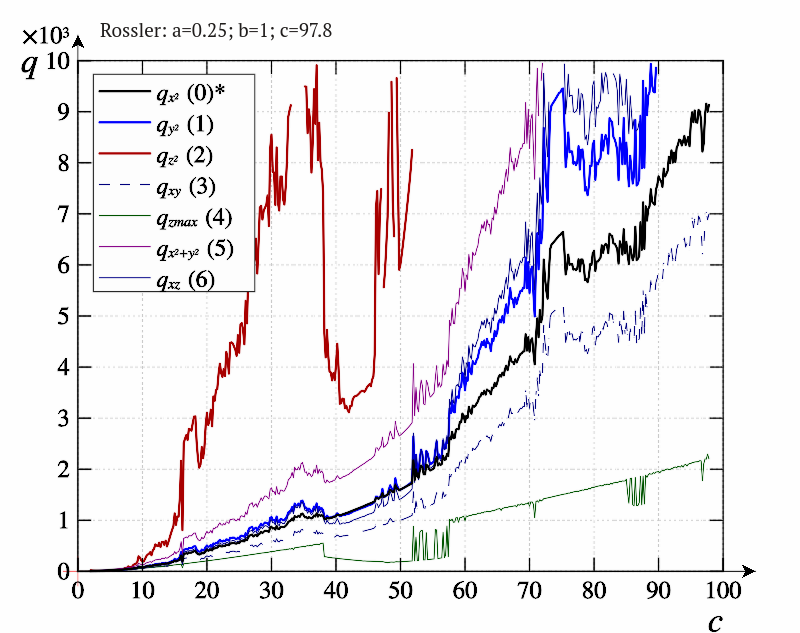
\includegraphics[width=0.49\textwidth]{p/cha/ross/ross_q-p_q.png}
  \hfill
  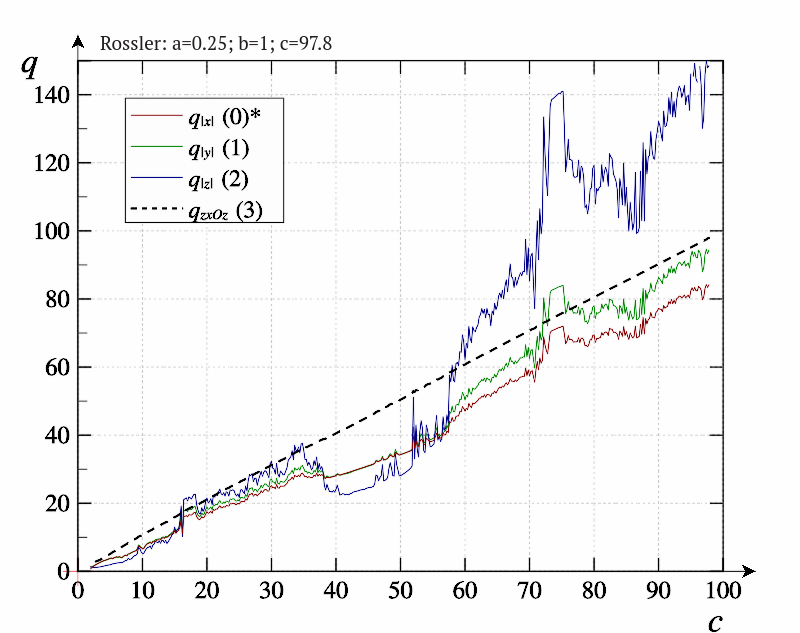
\includegraphics[width=0.49\textwidth]{p/cha/ross/ross_q-p_q1.png}
\end{center}
\caption{Розглянуті критерії для системи Ресслера}
\label{atu:f:ross_q}
\end{figure}

Як і слід було очікувати, велика частина критеріїв мало
придатна для застосування в методах ідентифікації. Незважаючи
на явні загальні тенденції в поведінці графіків, наявність
нерегулярних коливань не дозволяють розраховувати на прийнятну
точність. Кращі властивості демонструє критерій
$ q_{z \max{}} $, графік якого містить порівняно довгі прямі
ділянки. Однак, застосування цього критерію обмежено однією такою
ділянкою, межі якої залежать від інших параметрів системи.

Для прикладу розглянемо залежності критерію
$q_{x^2} $ від значень двох параметрів~(рис.~\ref{atu:f:ross_q_x2_ac_bc}).

\begin{figure}[htb!]
  \PicDouble{p/cha/ross/ross_pwr-x_a_c.png}{p/cha/ross/ross_pwr-x_b_c.png}
  \caption{Залежності $ q_{x^2}(a,c)$~(a) і $ q_{x^2}(b,c)$~(b) для системи Ресслера}
\label{atu:f:ross_q_x2_ac_bc}
\end{figure}

Складна і порізана структура отриманих поверхонь свідчить не
тільки про практично неможливу ідентифікацію одночасно двох
параметрів, а й про те, що досить малі похибки про визначенні
одного з них призводять до суттєвих помилок ідентифікації
іншого.

Залежності
$ q_{z \max{}} (a, c) $ і $ q_{z \max{}} (b, c) $ (рис.~\ref{atu:f:ross_q_zmax_ac_bc})
побудовані для області
параметрів, для якої не спостерігається суттєва зміна поведінки
критерію, показує кращі результати. Однак, навіть в цій області
відбуваються різкі ``провали'' графіка. Така поведінка може і не
привести в суттєвих помилок ідентифікації. Проте, при попаданні
однієї з моделей в область ``провалу'' процес ідентифікації
може бути порушений.

\begin{figure}[htb!]
  \PicDouble{p/cha/ross/ross_zmax_a_c.png}{p/cha/ross/ross_zmax_b_c.png}
  \caption{Залежності $q_{z \max{}}(a,c) $~(a) і $q_{z \max{}}(b,c)$~(b) для системи Ресслера}
\label{atu:f:ross_q_zmax_ac_bc}
\end{figure}

Спробуємо вивести більш придатний для задачі ідентифікації
критерій, виходячи з виду системи~(\ref{atu:eq:rossler}). Безпосередньо
параметр
$c$ входить тільки в останнє рівняння системи. Так як
розглядаються тільки режими, що проявляють стійку по Пуассону
динаміку, то при усередненні на великому інтервалі часу ліва
частина прагне до нуля. У правій частині є два параметри: $c$ і
$b$. Навіть для умов усереднення немає можливості визначити
обидва, але для ідентифікації тільки
$c$ введемо такий критерій:
%
\begin{equation}
  q_{xzOz} =
  \frac{ \overline{xz}}{ \overline{z}}.
  \label{atu:eq:ross_qzxOz}
\end{equation}

При фіксованих параметрах
$ a $ і
$ b $ графік
$q_{xzOz}(c)$ має близьку до лінійної залежність~(рис.~\ref{atu:f:ross_q}, правий графік, пунктирна крива).
Однак, застосування цього
критерію призводить до певних труднощів. Перш за все, наявність
дробової залежності вимагає окремого аналізу знаменника. З
аналізу аттрактора системи відомо, що
$ z> 0 \; \forall \; t> 0 $, тобто знаменник гарантовано не є нуль. При цьому
вид залежності
$z(t)$ характеризується різкими сплесками, між якими знаходяться
області, в яких
$ z \approx 0 $, що може привести до значних сплесків в значенні
критерію. Однак, ця ж величина
$z$ входить і в чисельник як множник, і якщо метод і параметри
усереднення в чисельнику і знаменнику однакові, то збурення
критерію будуть обмеженими.


% }}}2

\subsection{Тестова задача ідентифікації для системи Ресслера} % {{{2

Для синтезу системи ідентифікації була обрана група методів
``ql3rlWvnAAW'', критерій
$ q_{xzOz} $.
Використовувані значення параметрів:
$ a = 0.25 $,
$ b = 1 $,
$ c \in [3, 40] $.

Перш за все, розглянемо процес ідентифікації
в квазістаціонарному випадки, при повільної зміні
параметра~(\ref{atu:eq:po_t_ramp}),
$ p_0 = 10 $,
$ U_p = 20 $. Динаміка агентів і різних визначень
$ p_\mathrm{id} $ представлена на рис.~\ref{atu:f:ross_id_ramp}.


\begin{figure}[htb!]
  \PicDouble{p/cha/ross/ross_id-p_t_pi_ql3rlWvnAAW_ramp.png}{p/cha/ross/ross_id-p_t_p_ql3rlWvnAAW_ramp.png}
  \caption{Динаміка агентів~(a) і ідентифікованого значення~(b) для системи Ресслера за умови (\ref{atu:eq:po_t_ramp})}
  \label{atu:f:ross_id_ramp}
\end{figure}

Графіки динаміки агентів показують, що спостерігається коректний
``супровід'' агентами ідентифікованого параметра, за винятком
невеликої початкової ділянки, на якої усереднення критерію
на дає коректних результатів. Все залежності
$p_\mathrm{id} $ мають практично однакову динаміку,
що приводить до гарного наближення ідентифікованого параметра. При цьому
спостерігаються незначні, але різкі ``сплески'', викликані
аналогічним явищем для критерію. Доброю ознакою є те, що
немає помітних областей, в яких процес ідентифікації
порушується або помітно втрачає точність.

Розглянемо динамку процесу ідентифікації (рис.~\ref{atu:f:ross_id_sign})
в тому випадку, коли ідентифікований параметр зазнає різкі
скачки~(\ref{atu:eq:po_t_sign}),
$ p_0 = 21 $,
$ U_p = 7 $,
$ \omega_{in} = 0.01047 $.

\begin{figure}[htb!]
  \PicDouble{p/cha/ross/ross_id-p_t_pi_ql3rlWvnAAW_sign.png}{p/cha/ross/ross_id-p_t_p_ql3rlWvnAAW_sign.png}
  \caption{Динаміка агентів~(a) і ідентифікованого значення~(b) для системи Ресслера за умови (\ref{atu:eq:po_t_sign})}
\label{atu:f:ross_id_sign}
\end{figure}

Крім загальної працездатності методу ідентифікації слід
зазначити, що в даному випадку всі розглянуті способи визначення
$ p_\mathrm{id} $ дають результати, які практично неможливо розрізнити.

На рис.~\ref{atu:f:ross_id_sin} представлені аналогічні результати, але
в разі більш плавної зміни параметра~(\ref{atu:eq:po_t_sin}), при інших
рівних.


\begin{figure}[htb!]
  \PicDouble{p/cha/ross/ross_id-p_t_pi_ql3rlWvnAAW_sin.png}{p/cha/ross/ross_id-p_t_p_ql3rlWvnAAW_sin.png}
  \caption{Динаміка агентів~(a) і ідентифікованого значення~(b) для системи Ресслера за умови (\ref{atu:eq:po_t_sin})}
\label{atu:f:ross_id_sin}
\end{figure}

Принципових відмінностей не виявлено, середня похибка
ідентифікації в цьому випадку нижче, що досить очевидно.


% }}}2

\subsection{Вплив параметрів системи ідентифікації на похибку ідентифікації для системи Ресслера} % {{{2

Розглянемо вплив параметрів системи ідентифікації. Для даної
системи вибір правильного значення
$a_q$ особливо важливий, зважаючи на наявність різких імпульсів
в значенні критерію. Характерний вид такої залежності
представлено на рис.~\ref{atu:f:ross_q_t}.

\begin{figure}[htb!]
  \PicDouble{p/cha/ross/ross_id-p_t_q_ql3rlWvnAAW_sign.png}{p/cha/ross/ross_id-p_t_q_ql3rlWvnAAW_sin.png}
\caption{Характерний вид залежностей $ q_{xzOz} (t) $ для системи Ресслера за умов (\ref{atu:eq:po_t_sign})~(a) і (\ref{atu:eq:po_t_sin})~(b)}
\label{atu:f:ross_q_t}
\end{figure}

Незважаючи на наявність таких імпульсів, загальний
вид залежності похибки ідентифікації залишається
незмінним~(рис.~\ref{atu:f:ross_e_a_q}).
Так як більшість методів визначення
$p_\mathrm{id} $ дають близькі результати, на на цьому і наступних
графіках обмежимося п'ятьма. Зростання похибки ідентифікації
при
$a_q \to 0 $ обумовлено тим, що надлишкові фільтруючі властивості
критерію не дозволяють не тільки відреагувати, але й помітити
зміну динаміки системи. Зростання в правій частині графіка,
як і в попередніх тестових завданнях, обумовлені недостатнім
часом усереднення критерію.

\begin{figure}[htb!]
  \PicDouble{p/cha/ross/ross_id-p_a_q_ql3rlWvnAAW_sign.png}{p/cha/ross/ross_id-p_a_q_ql3rlWvnAAW_sin.png}
  \caption{Залежності $ \overline{e} (a_q) $ для системи Ресслера за умов (\ref{atu:eq:po_t_sign})~(a) і (\ref{atu:eq:po_t_sin})~(b)}
\label{atu:f:ross_e_a_q}
\end{figure}

Наступний параметр, що впливає на властивості системи
ідентифікації ---
$ q_\gamma $. Для сімейства методів ``ql3rlWvnAAW'' він застосовується
двічі. Перший раз, в складі значення
$W$, він визначає динаміку одного агента. Другий раз --- задає
рівень впливу агента на рівні координатора. На відміну від
методів ``Fq\ldots'' цей параметр не використовується при визначенні агентом
величини $p_e$. Отримані залежності
$\overline{e}(q_\gamma) $ представлені на рис.~\ref{atu:f:ross_e_q_gamma}.

\begin{figure}[htb!]
  \PicDouble{p/cha/ross/ross_id-p_q_gamma_ql3rlWvnAAW_sign.png}{p/cha/ross/ross_id-p_q_gamma_ql3rlWvnAAW_sin.png}
\caption{Залежності $\overline{e}(q_\gamma) $ для системи Ресслера за умов (\ref{atu:eq:po_t_sign})~(a) і (\ref{atu:eq:po_t_sin})~(b)}
\label{atu:f:ross_e_q_gamma}
\end{figure}

Обидва графіка демонструють збільшення похибки ідентифікації
при надмірній чутливості, тобто при
$q_\gamma \to 0$. Однак в подальшому поведінку графіків
розрізняються. Якщо параметр змінюється різко, що похибки
ідентифікації, пов'язані з недостатньою чутливістю, стають
малими, в порівнянні з похибками, зумовленими обмеженою
швидкістю зміни критерію, і залежність від
$q_\gamma$ практично відсутня. При менш яскраво вираженої динаміки
зміни параметра, з'являється як збільшення похибки через
недостатню чутливість, так і відмінність між застосовуваними
пошуковими координаторами методів. В першу чергу зростає
похибка ідентифікації у методів, які використовують
$p_c$, в другу --- у методів, які використовують ``глобальні'' оцінки.
Але в цілому, якщо виключити область надмірної
чутливості, вплив цього параметра незначний, що зумовлено
адаптаційними властивостями методу. Метод ql3rlWvnleW менш за інших
схильний втрачати точність при зростанні чутливості.

Вплив параметра
$v_f$ для методів, які використовують ансамбль агентів, перш за
все зумовлює динаміку точної настройки параметра, а не швидкість
реакції на різкі зміни параметра. Тому правий графік відповідних
залежностей (рис.~\ref{atu:f:ross_e_v_f}), показує більш значний вплив
цього параметра.

\begin{figure}[htb!]
  \PicDouble{p/cha/ross/ross_id-p_v_f_ql3rlWvnAAW_sign.png}{p/cha/ross/ross_id-p_v_f_ql3rlWvnAAW_sin.png}
\caption{Залежності $ \overline{e} (v_f) $ для системи Ресслера за умов (\ref{atu:eq:po_t_sign})~(a) і (\ref{atu:eq:po_t_sin})~(b)}
\label{atu:f:ross_e_v_f}
\end{figure}

Лівий графік свідчить про те, що при стрибкоподібному зміні
параметра виправданою стає велика швидкість переміщення
агентів, незважаючи на зменшення точності через надмірне
пересування агентів. Слід зазначити, що в даному прикладі
переміщення агентів обмежені. Без цього обмеження при зростанні
$ v_f $ спостерігається порушення стійкості пошуку.

Вплив коефіцієнта
$k_e$ (рис.~\ref{atu:f:ross_e_k_e}) в якійсь мірі має спільні риси
з впливом коефіцієнта
$v_f$. Відмінність полягає в тому, що
$k_e$ впливає не тільки на швидкість переміщення агентів, але
на їх рівноважну конфігурацію.

\begin{figure}[htb!]
  \PicDouble{p/cha/ross/ross_id-p_k_e_ql3rlWvnAAW_sign.png}{p/cha/ross/ross_id-p_k_e_ql3rlWvnAAW_sin.png}
\caption{Залежності $\overline{e}(k_e)$ для системи Ресслера за умов (\ref{atu:eq:po_t_sign})~(a) і (\ref{atu:eq:po_t_sin})~(b)}
\label{atu:f:ross_e_k_e}
\end{figure}

Як і для попереднього параметра, вплив цього коефіцієнта проявляється
значніше при плавній зміні параметра. І знову ж таки, без
штучного обмеження рухливості агентів високі величини
$k_e$ призводять до втрати стійкості пошуку.

Вплив параметра
$k_{nl}$ (рис.~\ref{atu:f:ross_e_k_nl})
відображає властивості множини агентів як ансамблю.

\begin{figure}[htb!]
  \PicDouble{p/cha/ross/ross_id-p_k_nl_ql3rlWvnAAW_sign.png}{p/cha/ross/ross_id-p_k_nl_ql3rlWvnAAW_sin.png}
\caption{Залежності $\overline{e} (k_{nl}) $ для системи Ресслера за умов (\ref{atu:eq:po_t_sign})~(a) і (\ref{atu:eq:po_t_sin})~(b)}
\label{atu:f:ross_e_k_nl}
\end{figure}

Малі значення величини
$k_{nl}$ призводять до того, що рух агентів стає практично
незалежним, при цьому конфігурація агентів поблизу шуканого
значення далека від оптимальної. І навпаки, збільшення
$k_{nl}$ перетворює ансамбль в сітку, з неминучим зростанням
похибки ідентифікації.

Наявність штучних обмежень на переміщення агентів призводить
до того, що вплив коефіцієнта
$k_{cl} $ стає мінімальним (рис.~\ref{atu:f:ross_e_k_cl}).

\begin{figure}[htb!]
  \PicDouble{p/cha/ross/ross_id-p_k_cl_ql3rlWvnAAW_sign.png}{p/cha/ross/ross_id-p_k_cl_ql3rlWvnAAW_sin.png}
\caption{Залежності $\overline{e}(k_{cl}) $ для системи Ресслера за умов (\ref{atu:eq:po_t_sign})~(a) і (\ref{atu:eq:po_t_sin})~(b)}
\label{atu:f:ross_e_k_cl}
\end{figure}

Більш того, при плавній зміні параметра його введення
лише погіршує якість ідентифікації, створюючи додаткову
нерівномірність в розподілі агентів. При стрибкоподібному зміні
ідентифікованого параметра несуттєве покращення пов'язано зі
збільшенням відстані між агентами, і більш швидкою реакцією
на стрибок параметра.


% }}}2




\subsection{Висновки} % {{{2

Результати моделювання процесів ідентифікації параметра ``$c$''
системи Ресслера, дозволяють в зробити наступні висновки:

\begin{itemize}

  \item
    Стандартний набір критеріїв має для цієї системи досить
    обмежене застосування.

  \item
    Використання критерію
    $ q_{xzOz} $ дозволяє побудувати працездатну систему ідентифікації.

  \item
    Група методів ql3rlWvnAAW показала свою добру працездатність, а
    швидкість ідентифікації при цьому в першу чергу визначається
    динамікою критерію.

  \item
    Параметри самої системи ідентифікації можуть змінюватися
    в досить широких межах без істотного збільшення похибки
    ідентифікації.

\end{itemize}


% }}}2


% }}}1

% vim: fdm=marker foldlevel=1 foldignore="%#" fdc=4 ft=tex
